\documentclass{article}
\usepackage[utf8]{inputenc}
\usepackage{amsmath, amsfonts, amsthm, amssymb, graphicx, geometry, lipsum}
\usepackage{hyperref}
\usepackage{indentfirst}
\usepackage[all,cmtip]{xy}
\usepackage{float}


\newtheorem{definition}{Definition}[section]
\newtheorem{lemma}{Lemma}[section]
\newtheorem{theorem}{Theorem}[section]
\newenvironment{theorem*}
 {\expandafter\def\expandafter\thetheorem\expandafter{\thetheorem*}\theorem}
 {\endtheorem}
\newtheorem{corollary}{Corollary}[theorem]
\newtheorem{proposition}{Proposition}[theorem]


\newcommand{\N}{\mathbb{N}}
\newcommand{\Z}{\mathbb{Z}}
\newcommand{\Q}{\mathbb{Q}}
\newcommand{\R}{\mathbb{R}}
\newcommand{\C}{\mathbb{C}}
\newcommand{\F}{\mathbb{F}}
\newcommand{\PP}{\mathbb{P}}
\newcommand{\HH}{\mathbb{H}}
\newcommand{\norm}[1]{\left\lVert #1 \right\rVert}
\newcommand{\innerp}[2]{\langle #1, #2 \rangle}

\DeclareMathOperator{\di}{d\!}




\title{Realization of planar configurations and polytopes\\
{\Large University of Toronto}}
\author{Haocheng Sun}
\date{Fall 2024}

\begin{document}
\maketitle


\section{Realization of (planar) configuration}

\begin{definition}
    Consider a finite set of points $V=\{v_1,\cdots,v_n\}$ and lines $E=\{e_1,\cdots,e_m\}\subset 2^V$. 
    A \underline{configuration} is defined as $\mathcal{C}=(V,E)$ where each pair $(v_i,e_j)$ indicates that point $v_i$ lies on the line $e_j$.
\end{definition}

\text{Remark}
\begin{itemize}
    \item What is the definition for a line here? A line here is a subset of $V$ that contain at least two points in $V$.
    For example, here is the picture of $V=\{v_1,v_2,v_3\}$ and $E=\{\{v_1,v_2\},\{v_1,v_3\},\{v_2,v_3\}\}$.
    \begin{figure}[H]
        \centering
        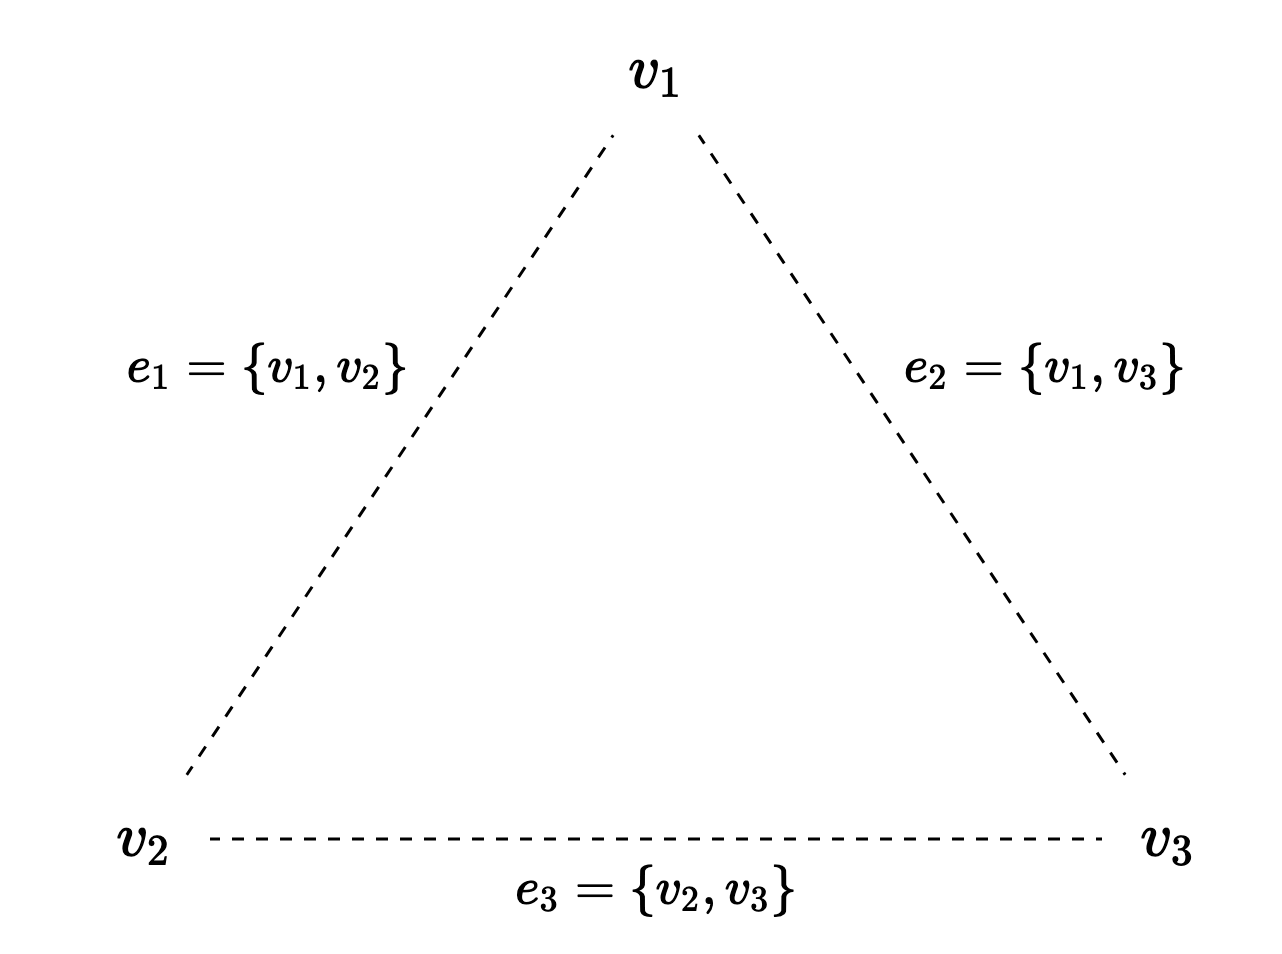
\includegraphics[scale=0.3]{images/Screenshot 2024-11-02 at 18.36.50}
        \caption{example1}
    \end{figure}
    \item Like the definition of topological space where we only need a set of points and some open sets. 
    It is an abstract structure, no need to embedded it into other spaces like $\R^n$.
    \item Through out this paper, we only consider planar configurations.
\end{itemize}

\begin{definition}
    For a configuration $\mathcal{C}=(V,E)$, we define a \underline{(affine) realization} as a map $$f:V\longrightarrow \mathbb{K}^2$$
    where $f(v_i)\in f(e_j)$ if and only if $v_i\in e_j$ for all $v_i\in V$ and $e_i\in E$. 
    In other words, the coordinate of each point are number in $\mathbb{K}$.
\end{definition}

\begin{definition}
    Given any field $\mathbb{K}$, we define \underline{the projective space} $\mathbb{K}\mathbb{P}^n$, also denoted as $\mathbb{P}^n(\mathbb{K})$ or $\mathbb{P}(\mathbb{K}^{n+1})$, as 
    the set of equivalence classes of $\mathbb{K}^{n+1} \setminus\{0\}$ under the equivalence relation $\sim$ defined by $x \sim y$ if there is a nonzero element $\lambda$ of $\mathbb{K}$ such that $x = \lambda y$.
    For each element in $\mathbb{K}\mathbb{P}^2$, we can write it as $[x_1,x_2,\cdots,x_n]$. 
\end{definition}

\text{Example}: Visualization of $\R\PP^2$.
\begin{itemize}
    \item In topology, we know that we can think of $\R\PP^2$ as gluing each pair of antipodal points of $S^2\subset\R^3$.
    \item In differential geometry, I studied that we can even realize $\R\PP^2$ smoothly as a surface inside $\R^3$, possibly with self-intersections. This can be shown by the famous Boy's surface.
    \begin{figure}[H]
        \centering
        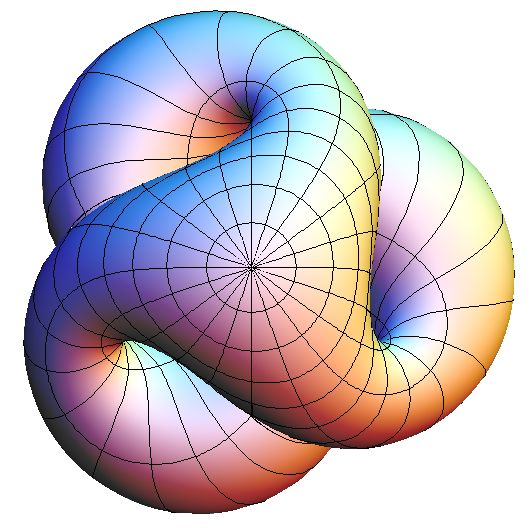
\includegraphics[scale=0.3]{images/133c07829c226ed20e71f18663d63e1b}
        \caption{boy's surface in $\R^3$}
    \end{figure}
    \item For here, I have a better visualization. \cite{uwashington}
    Pretend that the $w=1$ plane is the projective plane. There is a pair of parallel lines lying in this plane: $ax+by+c_1=0$ and $ax+by+c_2=0$. These two lines don't intersect in the ordinary sense, but their intersection in the projective plane is a point at infinity. Let's see what the intersection of their homogeneous counterparts is. Every point on the $w=1$ plane corresponds to a 3D line through that point and the origin. The two parallel lines thus correspond to two planes. The planes intersect in a line, parallel to the first two, but passing through the origin (and thus lying in the w=0 plane). Back in the projective system, this line corresponds to the point at infinity which is the projective intersection of the original two lines.
    \begin{figure}[H]
        \centering
        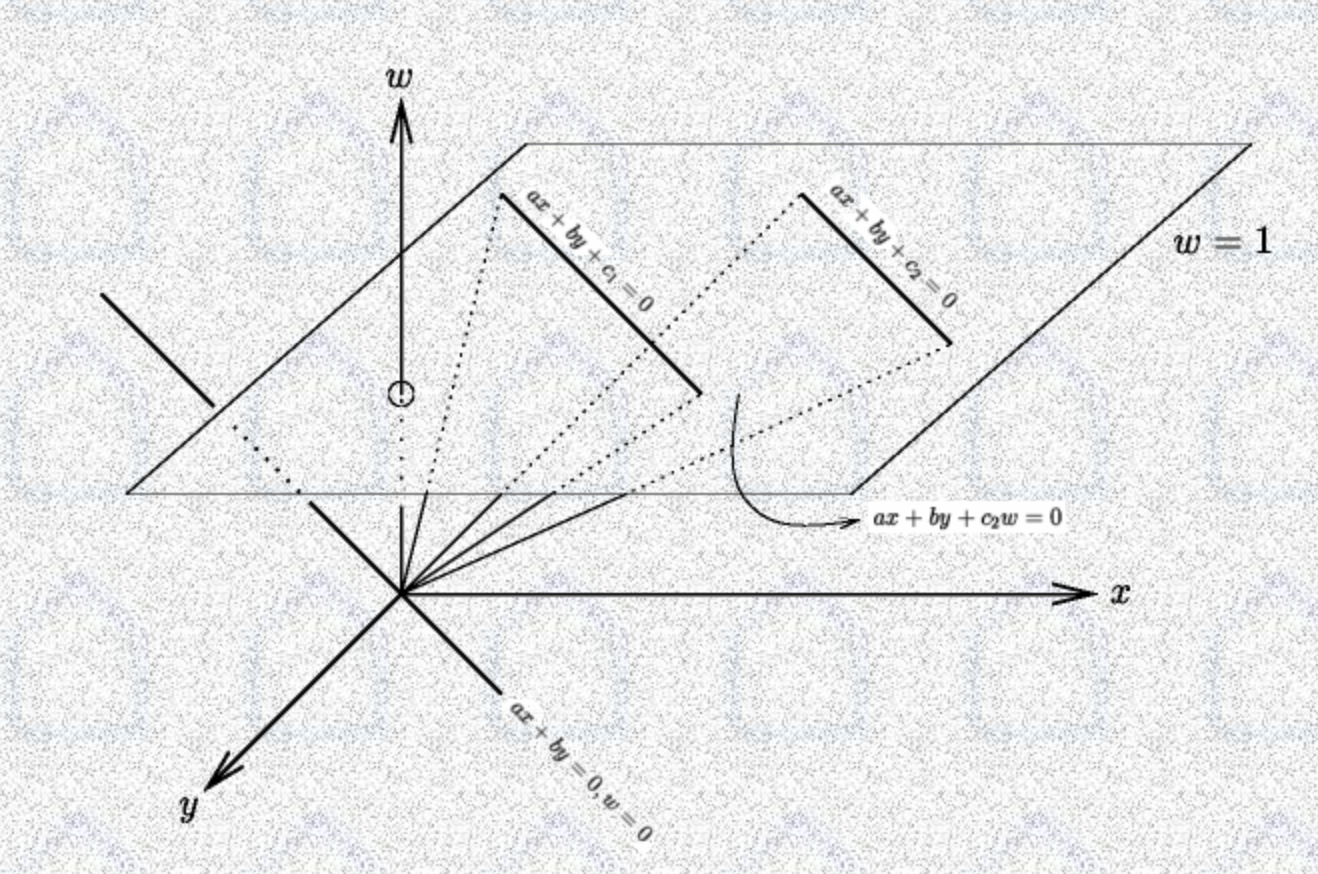
\includegraphics[scale=0.3]{images/Screenshot 2024-11-03 at 16.20.36}
        \caption{lines in projective plane}
    \end{figure}
    In two dimensions, the projective plane is the ordinary real plane augmented by a "line at infinity" r. 
    For each direction d (and -d), there is associated a point at infinity $d_{\infty}=d_{-\infty}$. This point is considered to lie on every line parallel to d. The locus of these points forms the line r.
    \begin{figure}[H]
        \centering
        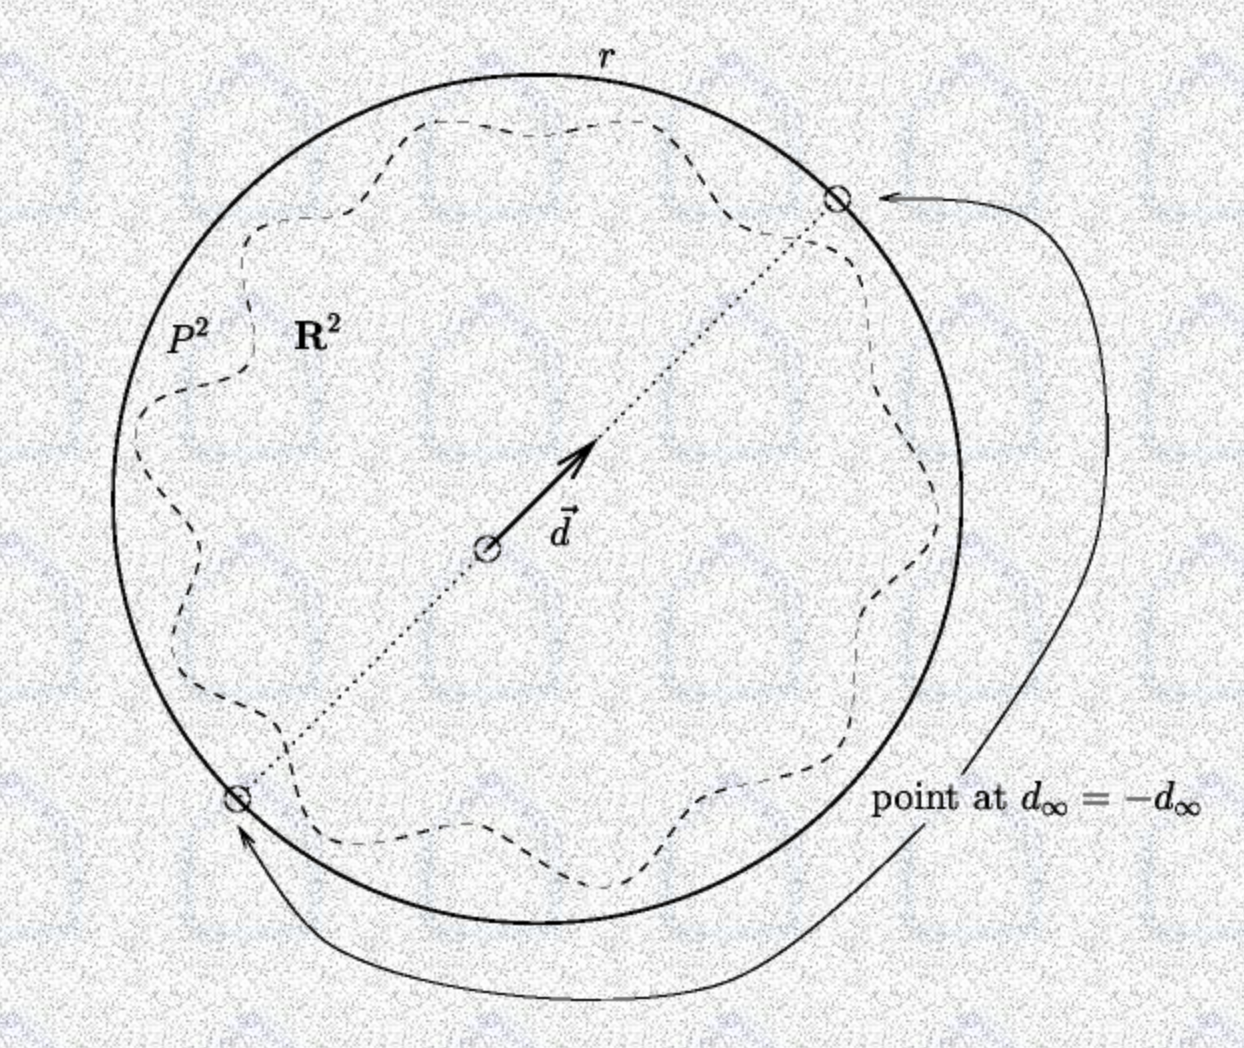
\includegraphics[scale=0.3]{images/Screenshot 2024-11-02 at 23.54.07}
        \caption{another visualization of $\R\PP^2$}
    \end{figure}
\end{itemize}

\begin{definition}
    For a configuration $\mathcal{C}=(V,E)$, we define a \underline{(projective) realization} as a map $$f:V\longrightarrow \mathbb{K}\mathbb{P}^2$$
    where $f(v_i)\in f(e_j)$ if and only if $v_i\in e_j$ for all $v_i\in V$ and $e_i\in E$. 
    We should notice that the realization is dependent on the field $\mathbb{K}$.
\end{definition}

\text{Remark}
\begin{itemize}
    \item Why we need to use projective space instead of the affine space $\mathbb{K}^2$? 
    Of course we can use this space. For our example1, we define $f(v_1)=(1,1)$, $f(v_2)=(0,0)$ and $f(v_3)=(2,0)$,
    we can easily realize it on our Euclidean plane $\R^2$, it becomes a discrete trangle. 
    But if we try to set $f(v_i)=\infty$, here comes the issue. So instead, in order to avoid this issue, we use prjective plane. Another good aspect is in projective geometry, all pairs of distinct lines intersect at a unique point, and all pairs of distinct points determine a unique line. 
    \item We can also consider realization of $\mathcal{C}$ over other fields, such as $\Q$, $\C$, or finite fields $\mathbb{F}_q$. 
    Here is a natural question: Is it true that configurations realizable over $\C$ are also realizable over $\R$? What about $\R$ versus $\mathbb{F}_q$? What about different finite fields? The answers to all these questions turns out to be a “NO”.
\end{itemize}

\subsection{Fano configuration}

\begin{definition}
    Consider this configuration: Given 7 points $V=\{v_1,v_2,v_3,v_4,v_5,v_6,v_7\}$ and lines as $\{\{v_1,v_6,v_2\},\{v_2,v_4,v_3\},\{v_3,v_5,v_1\},\{v_1,v_7,v_4\},\{v_2,v_7,v_5\},\{v_3,v_7,v_6\},\{v_4,v_5,v_6\}\}$. 
    This is called \underline{Fano configuration}.
\end{definition}

\begin{lemma}
    The projective plane $\mathbb{F}_2\mathbb{P}^2$ is isomorphic to the set of 1-dim subspaces of $\mathbb{F}_2^3$.
\end{lemma}
\begin{proof}
    Easy. I will prove this result for any field $\mathbb{K}$. In the definition of $\mathbb{K}\mathbb{P}^2$, 
    each equivalent class is a span of a none zero vector in $\mathbb{K}^{3}$ without the origin. This correspond to a 1-dim subspace.
\end{proof}

\begin{theorem}
    The fano configuration can be (projective) realized over $\mathbb{F}_2$. But it cannot be (affine) realized over $\mathbb{F}_2$.
\end{theorem}
\begin{proof}
    Easy, by using the lemma above. We know that $$\F_2\PP^2=\{(0,0,1),(0,1,0),(1,0,0),(0,1,1),(1,0,1),(1,1,0),(1,1,1)\}$$ 
    Recall, for any field $\F$, each element in $\F\PP^2$ correspond to a line passing origin in $\F^3$. But what is a line in $\F\PP^2$?
    We defined a line in $\F\PP^2$ to be something of the form $$\{[x_1,x_2,x_3]\in \F\PP^2:\alpha_1x_1+\alpha_2x_2+\alpha_3x_3=0, \alpha_1,\alpha_2,\alpha_3\text{ not all zero}\}$$
    \begin{figure}[H]
        \centering
        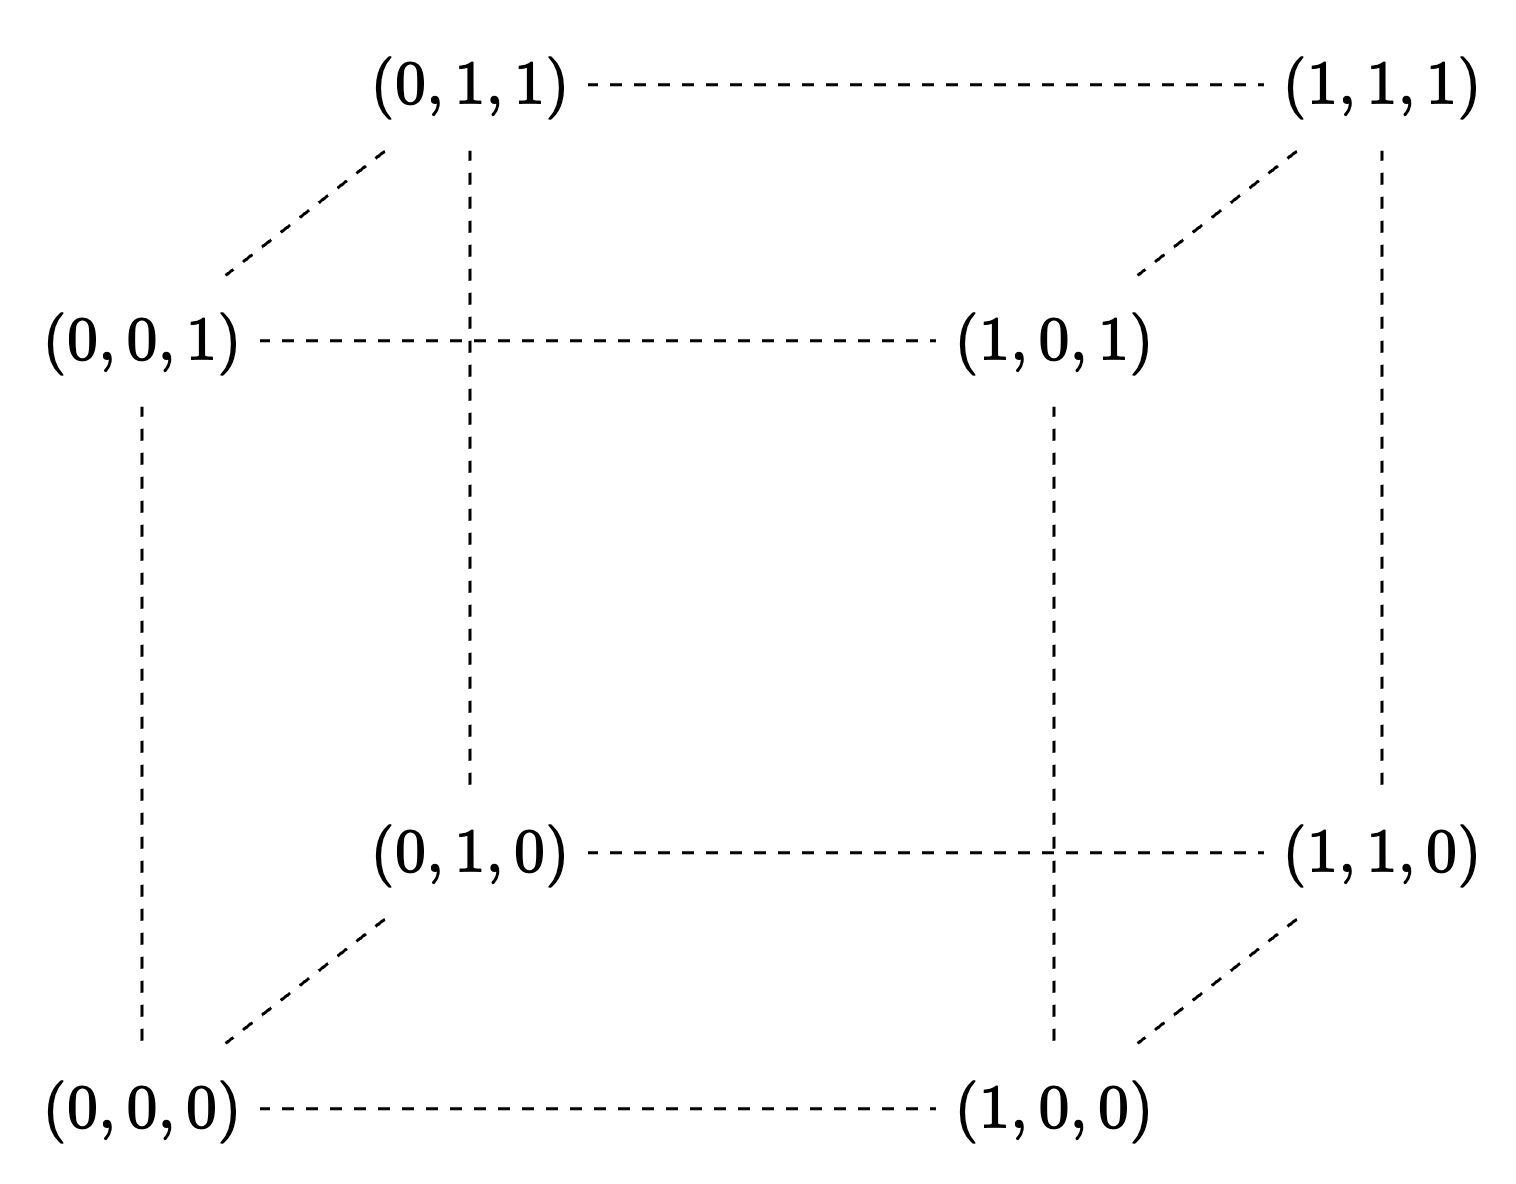
\includegraphics[scale=0.3]{images/Screenshot 2024-11-02 at 22.15.19}
        \caption{picture of $\F_2^3$}
    \end{figure}
    In the case of $\F=\F_2$, $(\alpha_1,\alpha_2,\alpha_3)$ has exactly 7 cases.
    \begin{align*}
        & (\alpha_1,\alpha_2,\alpha_3) = (1,1,1)\text{ so } (x_1,x_2,x_3)= (0,1,1),(1,0,1),(1,1,0)\\
        & (\alpha_1,\alpha_2,\alpha_3) = (1,1,0)\text{ so } (x_1,x_2,x_3)= (0,0,1),(1,1,0),(1,1,1)\\
        & (\alpha_1,\alpha_2,\alpha_3) = (1,0,1)\text{ so } (x_1,x_2,x_3)= (0,1,0),(1,0,1),(1,1,1)\\
        & (\alpha_1,\alpha_2,\alpha_3) = (0,1,1)\text{ so } (x_1,x_2,x_3)= (1,0,0),(0,1,1),(1,1,1)\\
        & (\alpha_1,\alpha_2,\alpha_3) = (1,0,0)\text{ so } (x_1,x_2,x_3)= (0,1,1),(0,1,0),(0,0,1)\\
        & (\alpha_1,\alpha_2,\alpha_3) = (0,1,0)\text{ so } (x_1,x_2,x_3)= (0,0,1),(1,0,0),(1,0,1)\\
        & (\alpha_1,\alpha_2,\alpha_3) = (0,0,1)\text{ so } (x_1,x_2,x_3)= (1,1,0),(1,0,0),(0,1,0)\\
    \end{align*}
    This is exactly the fano configuration.\\
    For the second part, just notice $\mathbb{F}_2^2$ has only 4 elements.
\end{proof}

\begin{lemma}[Gallai–Sylvester theorem]
    Let $X\subset \R^2$ be a finite set of points, not all on the same line. Then there exists a line containing exactly two points in $X$.
\end{lemma}

\begin{lemma}
    A projective plane over a field, does contain the Fano configuration if and only if the characteristic of the field is two.
\end{lemma}
\begin{proof}
    Left as homework.
\end{proof}

\begin{theorem}
    The fano configuration cannot be (projective) realized over $\R$. It also cannot be (affine) realized over $\R$.
\end{theorem}
\begin{proof}
    For the second part. Suppose we can. Then by the Gallai–Sylvester theorem above, there exists a line containing exactly two points, this is a contradiction.
\end{proof}

\text{Remark}
\begin{itemize}
    \item In many other books, the fano configuration is shown by the following picture. Fano configuration cannot be realized over $\R$ means there is no way to 'straighten' the middle circle.
    \begin{figure}[H]
        \centering
        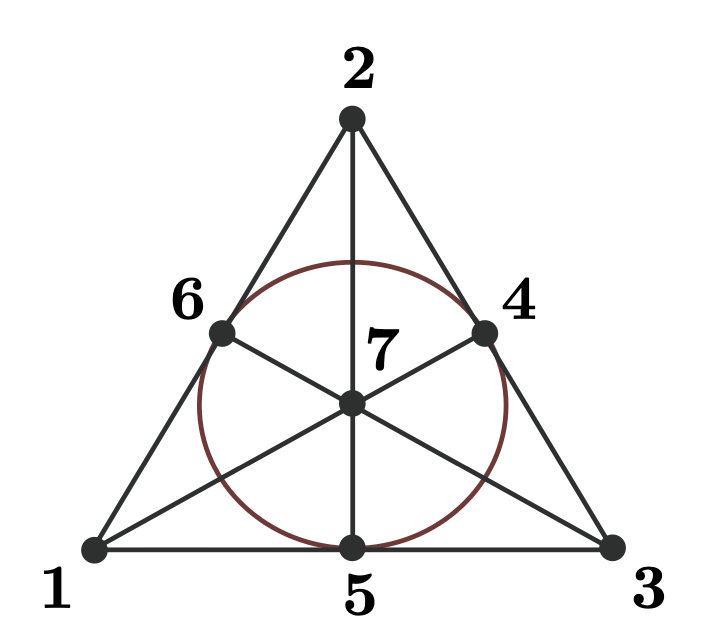
\includegraphics[scale=0.3]{images/Screenshot 2024-11-02 at 22.34.15}
        \caption{illustration of fano configuration}
    \end{figure}
    \item Fun fact. We define an automorphism of this configuration to be any permutation of points and lines that preserves
    the incidence relation. We denote $\mathcal{F}$ to be the fano configuration. Then $$Aut(\mathcal{F})\cong GL_3(\mathbb{F}_2)$$
    The simple group of order 168. \cite{dummit2003}
\end{itemize}


\subsection{Perles configuration}

\begin{definition}
    Consider 9 points $\{v_1,\cdots,v_9\}$ and ten lines below
    \begin{align*}
        \{&\{v_1,v_2,v_3,v_4\},\{v_1,v_6,v_7\},\{v_1,v_5,v_9\},\{v_8,v_5,v_2\},\{v_8,v_6,v_3\},\{v_8,v_7,v_4\},\\
        &\{v_9,v_5,v_1\},\{v_9,v_6,v_2\},\{v_9,v_7,v_3\},\{v_4,v_6,v_5\}\}
    \end{align*}
    This system is called \underline{Perles configuration}, denoted as $\mathcal{P}$.
\end{definition}

\begin{theorem}
    The perles configuration can be (affine) realized over $\R$. It also can be (projective) realized over $\R$.
\end{theorem}

\begin{proof}
    Let us consider the realization $f:V\longrightarrow \R^2$. This can be shown by the following picture. 
    \begin{figure}[H]
        \centering
        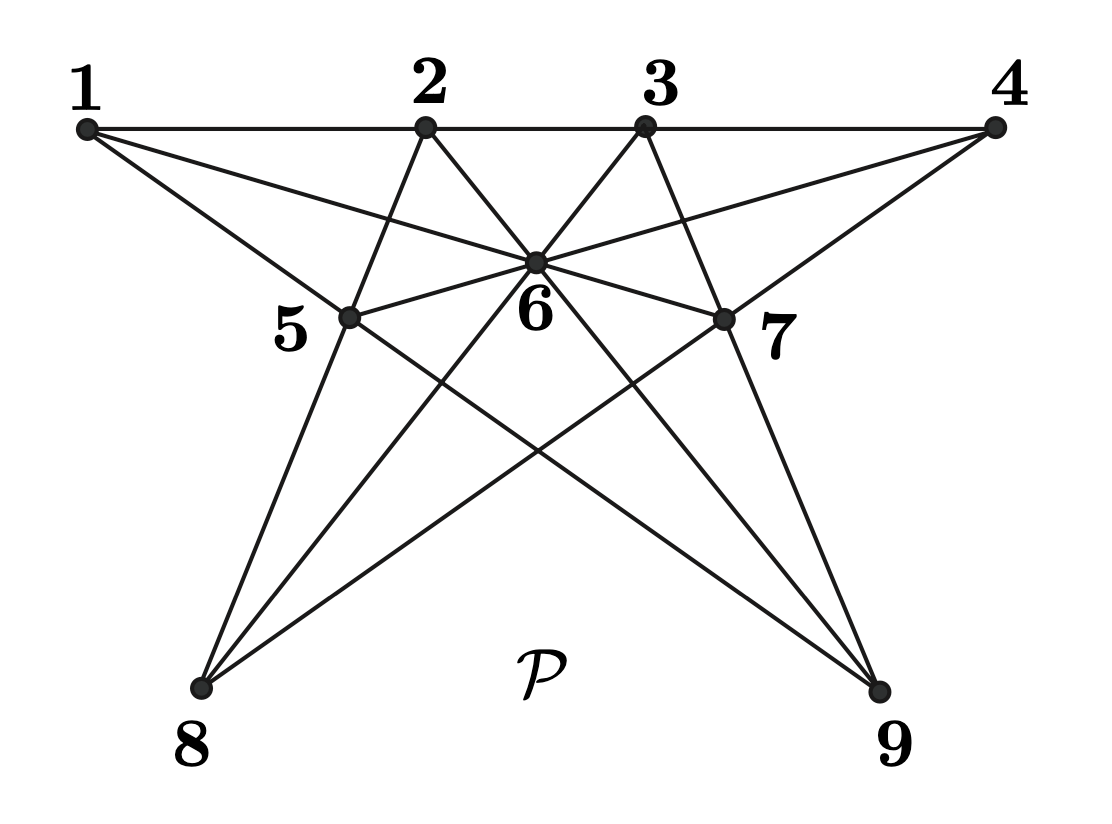
\includegraphics[scale=0.3]{images/Screenshot 2024-11-02 at 23.02.41}
        \caption{realization of perles configuration on $\R^2$}
    \end{figure}
    Now consider the map $\Phi: \R^2 \longrightarrow \R\PP^2;$ $(x_1,x_2)\longrightarrow[x_1,x_2,1]$. We can check that by composing this injective map, $\Phi\circ f$ is the realization from $V$ to $\R\PP^2$.
\end{proof}


\begin{theorem}
    The perles configuration cannot be (projective) realized over $\Q$.
\end{theorem}

\begin{proof}
    First, we can send the line $(1234)$ to the line at infinity by a projective linear transformation. Recall the definition of projective linear transformation: 
    \begin{align*}
        A_{3\times 3} : \mathbb{K}\mathbb{P}^2 & \longrightarrow \mathbb{K}\PP^2\\
        [x_1,x_2,x_3] & \longrightarrow [x_1',x_2',x_3']\text{ where } \vec{x}'=A\vec{x}
    \end{align*}
    For any line in $\mathbb{K}\PP^2$, it correspond to a plane $ax+by+cz=0$ in $\R^3$, we can use a to send this plane to the plane $z=0$ which correspond to the infinity line in $\mathbb{K}\PP^2$. 
    By previous observation, after the trasformaton, the line $(58)$, $(69)$ are parallel, the line $(78)$, $(5,6)$ will be parallel. Now just consider the pentagon $[56789]$, as following, notice also $(79)$, $(68)$ must be parallel
    \begin{figure}[H]
        \centering
        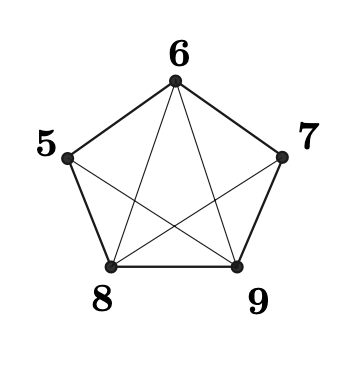
\includegraphics[scale=0.5]{images/Screenshot 2024-11-03 at 15.03.07}
        \caption{pentagon $[56789]$ after transformation}
    \end{figure}
    We then simply do a transformation to make the pentagon becomes following: (here we must assume the pentagon in the picture above has rational coordinates)
    \begin{figure}[H]
        \centering
        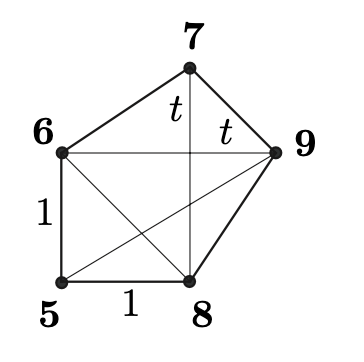
\includegraphics[scale=0.5]{images/Screenshot 2024-11-03 at 15.07.07}
        \caption{pentagon $[56789]$ after second transformation}
    \end{figure}
    By simple geometry, $t=-\frac{\sqrt{5}+1}{2}$ or $t=\frac{\sqrt{5}+1}{2}-1$. 
    To summarize, if perles configuration has a rational realization, there would be a rational projective linear map into a nonrational arrangement, a contradiction. 
    So we proved that it has no (projective) realization over $\Q$. For nonrealizable (affine) over $\Q$, proof is almost the same. We assume it has a rational realization, and use $\Phi:(x_1,x_2)\longrightarrow[x_1,x_2,1]$.
\end{proof}

\text{Remark:}
    \begin{itemize}
        \item So there is some configuration, that however we realize it on the Euclidean plane, we can never get all rational coordinates!
        \item In the 1960's, Grunbaum conjectured that Perles' construction is the smallest: any planar configuration on eight or fewer points if it is realizable with real coordinates in the plane, it is also realizable with rational coordinates. 
        Surprisingly, a professor at UBC gave a proof for this conjuecture this summer! \cite{solymosi2024}I am not sure if this is the first proof. 
        \item A natural question arises: What about polygons? If we can strech it without destroying its topological structure, can we put all vetices in rational coordinates?
    \end{itemize}


\section{Realization of polytope}

\begin{definition}
    The most familiar definition of a polytpoe $P\subset \R^n$ is define $P:=conv(S)$ where $S$ is a finite set of points. Equivalently, we can define it as the intersection of finitely many halfspaces but here we require the intersection to be bounded.
\end{definition}
\text{Remark:}
\begin{itemize}
    \item Like topological spaces and our point-line configuration before, we want an intrinsic structure.
\end{itemize}

\begin{definition}
    The \underline{face lattice} of a polytope is a structured way of organizing and representing all the faces of a polytope in terms of their inclusion relationships. It captures the hierarchical structure of faces in a polytope, from the lowest-dimensional faces (vertices) to the highest (the polytope itself).
    \begin{figure}[H]
        \centering
        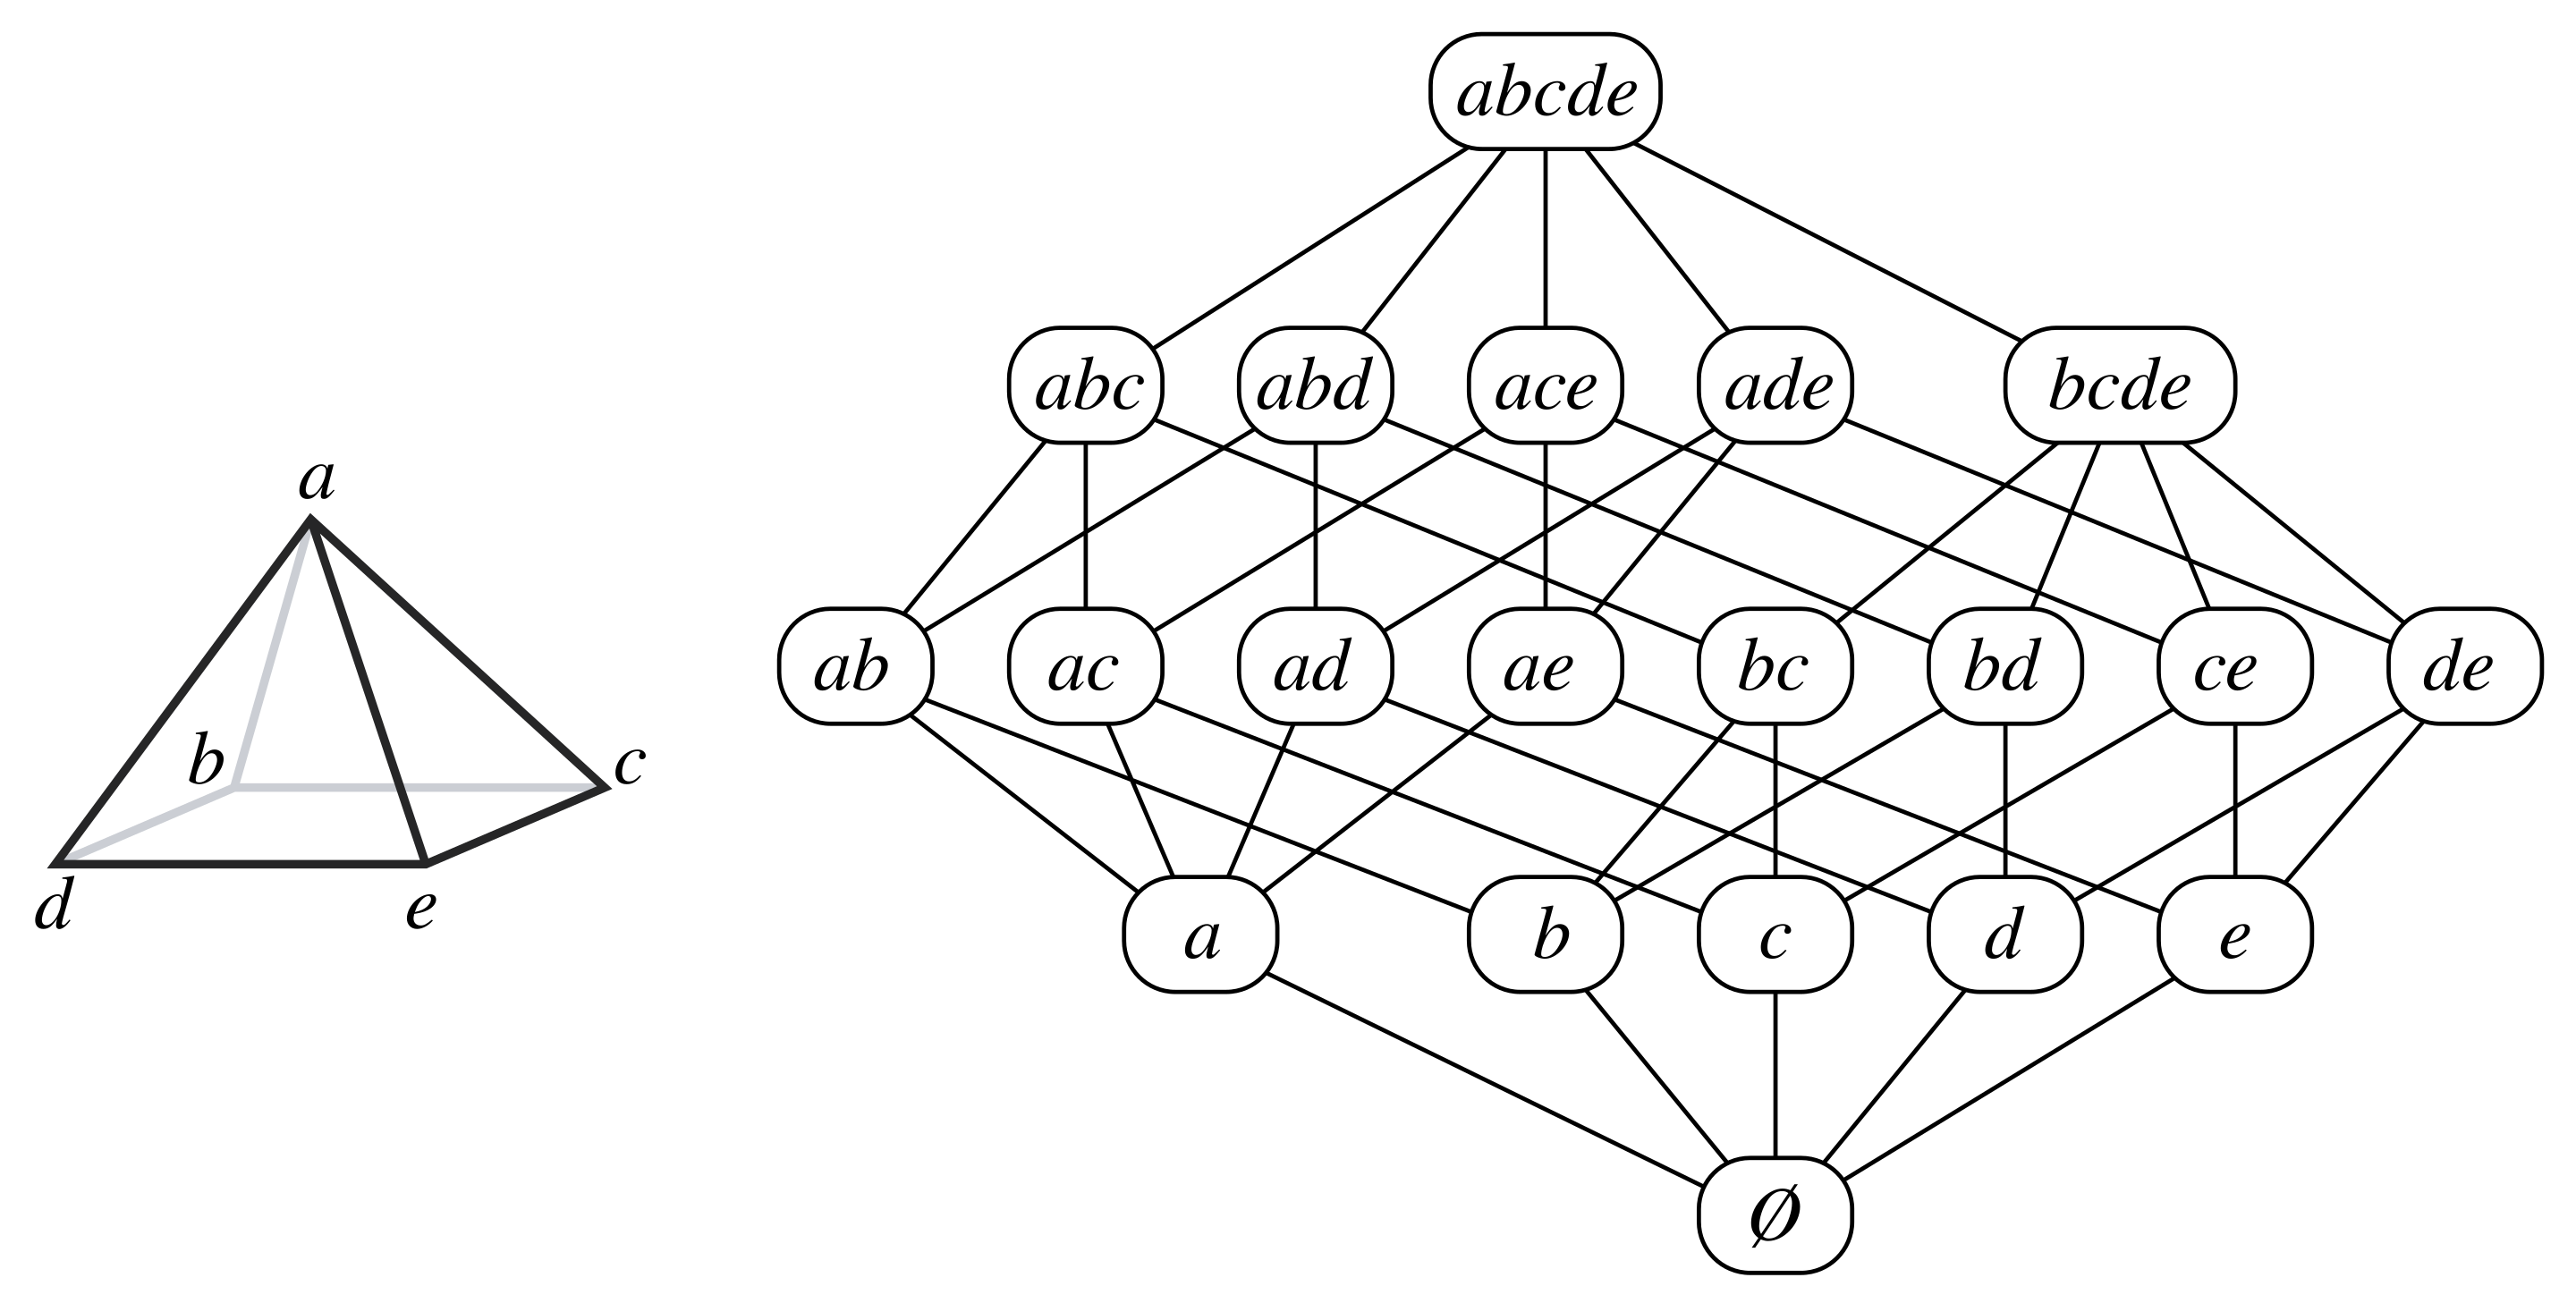
\includegraphics[scale=0.1]{images/Pyramid_face_lattice.svg.png}
        \caption{Pyramid face lattice}
    \end{figure}
    We say two polytopes are \underline{combinatorically equivalent} if they have the same face lattice.
\end{definition}

\begin{definition}
    We define a realization of a face lattice is to find a polytope in $\R^n$ which has this face lattice.
    When we say realization of a polytope, we mean realization of its face lattice.
\end{definition}

\begin{theorem*}[Perles, Mnev]
    There exists a polytope $P \subset \R^d$ which cannot be realized over $\Q$. Moreover, there exists a polytope $P \subset \R^d$ which cannot be realized over any finite extension of $\Q$.
\end{theorem*}


\section{A glimpse of universality}
Following venerable traditions for example from Algebraic Geometry (where one speaks of “mod- uli spaces”) it is natural and profitable to study not only special realizations for discrete-geometric structures such as configurations, polytopes. 
We want to study the space of all realizations which is known as the realization space of the structure.

\begin{theorem*}[Grunbaum]
    The realization space of any configuration, polytope or polyhedral surface is a semi-algebraic set.
\end{theorem*}

\text{Remark:}
\begin{itemize}
    \item For what is a semi-algebraic set, why it is a semi-algebraic set, what is realization of polyhedral surface, read the article in the reference.\cite{ziegler2007}
\end{itemize}

\begin{thebibliography}{9}

    \bibitem{pak2010} 
    I. Pak, 
    \textit{Lectures on Discrete and Polyhedral Geometry}, 
    April 20, 2010.
    
    \bibitem{dummit2003} 
    D. S. Dummit and R. M. Foote, 
    \textit{Abstract Algebra}, 
    Third Edition, 
    University of Vermont.
    
    \bibitem{uwashington} 
    \textit{Projective Transformations}, 
    available online at \url{https://courses.cs.washington.edu/courses/cse557/97wi/notes/xforms/projective.html}.
    
    \bibitem{solymosi2024} 
    J. Solymosi, 
    \textit{On Perles' Configuration}, 
    arXiv preprint arXiv:2408.09370, August 18, 2024.
    
    \bibitem{ziegler2007} 
    G. M. Ziegler, 
    \textit{Non-rational Configurations, Polytopes, and Surfaces}, 
    Inst. Mathematics, MA 6-2, TU Berlin, October 24, 2007; revised November 16, 2007.
    
    \end{thebibliography}
    
\end{document}